\chapter{Model Application Workflow}

This chapter presents the practical application of the proposed pricing model. The goal of this chapter is to present the workflow of the model on anonymized real-world data, from data preparation through demand forecasting to price recommendation, and to discuss selected design choices and their implications, limitations and scopes for possible improvements. The model is applied to a selected segment of apartments in the analyzed market, and the resulting price recommendations are compared to historical pricing decisions to evaluate the model's performance and potential benefits for accommodation providers. The full Python implementation, including the dataset and all source files required to reproduce the results, is provided in Appendix~\ref{app:code}.

\section{Input data}

The proposed model is based on historical reservation data, which are commonly available to accommodation providers through booking systems or other data sources. The dataset used in this chapter consists of 3787 anonymized, real-world reservation records collected from a booking platform for a segment of 13 selected Prague apartments spanning a period of 394 days from April 28th 2024 to May 27th 2025. The dataset includes reservations made for stays during this period, providing a view of booking patterns and price levels in the analyzed market segment. Each record in the dataset corresponds to a single reservation and contains relevant information about the booking readily available to the accommodation provider. The data required for the application of the model include:
\begin{itemize}
    \item \textbf{Apartment ID}: Unique identifier assigned to each apartment for which the reservation was made
    \item \textbf{Check-in date}: Date when the guest is expected to arrive
    \item \textbf{Check-out date}: Date when the guest is expected to depart
    \item \textbf{Number of guests}: Total number of guests included in the reservation
    \item \textbf{Price per night}: Price paid by the guest for each night of the stay
\end{itemize}

Additional information, such as the booking date, can also be included and later used to improve demand prediction. In addition to reservation data, the model requires basic information about the accommodation units themselves, such as their maximum capacity.

\section{Data preprocessing}
The model is designed around time-series containing daily demand and price data. The reservation data represent a time interval and are therefore transformed into the daily time series format, which serves as the primary input for the demand forecasting and price-setting components of the model. This transformation involves aggregating the reservation data to calculate daily demand in terms of beds sold and the corresponding average bed price in the analyzed period.

For illustration, a simplified example of the transformation process is shown in Tables~\ref{tab:reservation_example} and~\ref{tab:daily_time_series_example} on a subset of the real data.

\begin{table}[ht]
    \centering
    \begin{tabular}{|c|c|c|c|c|c|}
        \hline
        Apartment ID & Check-in Date & Check-out Date & Guests & Price per Night \\
        \hline
        0            & 11-17         & 11-20          & 2      & 3564.02         \\
        1            & 11-18         & 11-20          & 2      & 2504.67         \\
        \hline
    \end{tabular}
    \caption{Example of reservation data}
    \label{tab:reservation_example}
\end{table}

\begin{table}[ht]
    \centering
    \begin{tabular}{|c|c|c|c|}
        \hline
        Date  & Beds Sold & Average Bed Price \\
        \hline
        11-17 & 2         & 1782.01           \\
        11-18 & 4         & 1517.18           \\
        11-19 & 4         & 1517.18           \\
        \hline
    \end{tabular}
    \caption{Example of aggregated daily time series data}
    \label{tab:daily_time_series_example}
\end{table}

\section{Properties of Model Variables}

The constructed time series is enriched by derived variables. The occupancy rate $o_t$ and relative price index $r_t$, as defined in Chapter~2, are constructed from the aggregated time series. The occupancy rate measures demand relative to capacity, while the relative price index normalizes price levels across apartments and time. The development of these variables over time is visualized in Figure~\ref{fig:timeseries_basic}. The figure illustrates the presence of seasonal patterns in both demand and price, and outlining their co-movement. This relationship is further highlighted in Figure~\ref{fig:price_demand}, which shows a positive dependence between the observed occupancy rate and relative price index. The moderate strength of this relationship is reflected in the Pearson correlation coefficient $\rho = 0.583$, although the relationship is not strictly linear and is better approximated by a nonlinear trend.

\begin{figure}[ht]
    \centering
    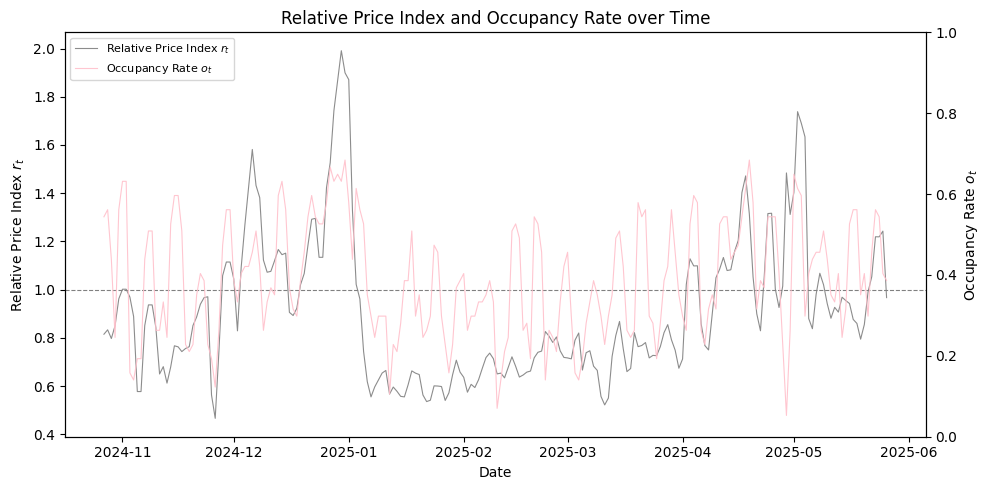
\includegraphics[width=1\textwidth]{figures/timeseries_basic.png}
    \caption{Time series of occupancy rate and relative price index.}
    \label{fig:timeseries_basic}
\end{figure}

\begin{figure}[ht]
    \centering
    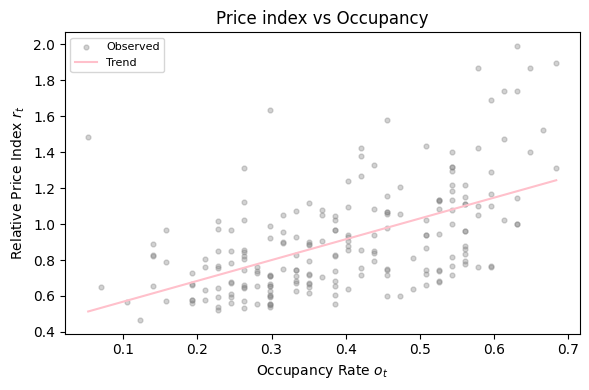
\includegraphics[width=0.6\textwidth]{figures/price_occupancy.png}
    \caption{Observed relationship between occupancy rate and relative price index.}
    \label{fig:price_demand}
\end{figure}

\section{Demand Forecasting}
To forecast future occupancy levels, a SARIMA model was fitted to the historical occupancy time series. Model parameters were selected automatically using the Akaike Information Criterion (AIC) through a stepwise search procedure.

The selected model corresponds to $\mathrm{SARIMA}(2,1,1)(1,0,2)_7$, capturing both short-term dynamics and weekly seasonal patterns in the data, with strong seasonal autoregressive component (approximately 0.99) that reflects the dependence of occupancy on values observed one week earlier. The inclusion of first-order differencing ($d=1$) indicates that the occupancy series exhibits non-stationary behavior, which is accounted for by modeling changes in occupancy over time. This is consistent with typical booking patterns in short-term accommodation markets.

The forecasted occupancy rates for the test period are visualized in Figure~\ref{fig:sarima_forecast}. The model captures the overall trend and seasonal fluctuations in demand, although some deviations from actual values are observed, particularly during periods of high volatility. An evaluation of forecast accuracy is presented in Section~\ref{sec:results}.

\begin{figure}[ht]
    \centering
    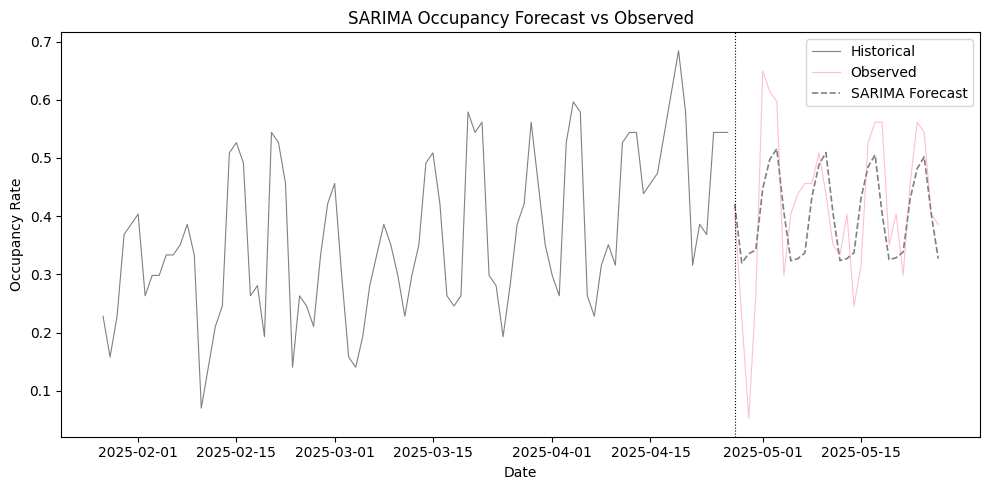
\includegraphics[width=1\textwidth]{figures/demand_prediction.png}
    \caption{SARIMA model forecast of occupancy rates compared to actual values.}
    \label{fig:sarima_forecast}
\end{figure}

\section{Estimation of Occupancy–Price Distribution}
The historical sample used for the price estimation stage consists of pairs $(o_t, r_t)$ constructed from the observed time series. This sample forms the empirical basis for estimating the relationship between occupancy and pricing. To capture this relationship, a joint probability density function of occupancy and relative price is estimated using a non-parametric Kernel Density Estimation (KDE) approach.

The estimation is performed using a Gaussian kernel applied to the historical sample, implemented via the \texttt{gaussian\_kde} function from the SciPy library \cite{2020SciPy-NMeth} with default automatic selection of the bandwidth parameter using Scott's rule.

The resulting estimated density function $\hat{f}_{O,R}(o, r)$ is visualized in Figure~\ref{fig:kde_density}, which shows the joint distribution of occupancy and relative price based on the historical data.


\begin{figure}[ht]
    \centering
    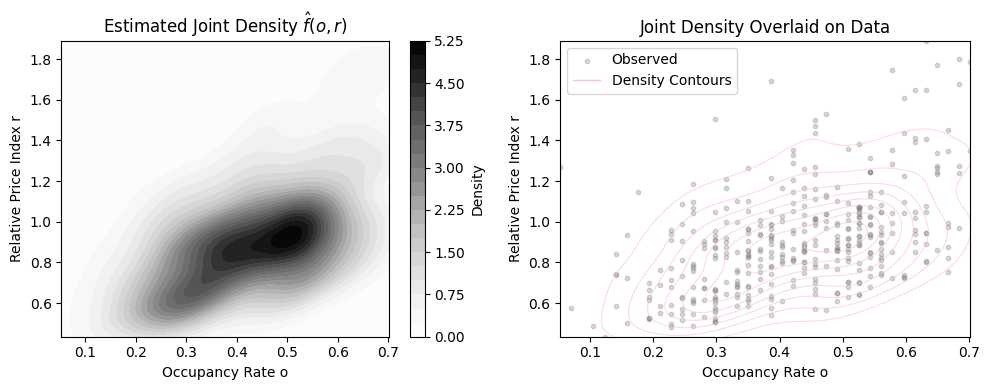
\includegraphics[width=1\textwidth]{figures/estimated_density.png}
    \caption{Estimated joint density of occupancy and relative price.}
    \label{fig:kde_density}
\end{figure}

The estimated density reflects historical pricing behavior under varying demand conditions and serves as the basis for deriving conditional price recommendations in the next step. For a given occupancy level, a relatively wide range of relative price indices can be observed. For example, at an occupancy level of $o=0.4$, the conditional mean of the relative price index is $\mathbb{E}[R \mid O=0.4] \approx 0.903$, with a standard deviation of $\sigma_{R \mid O=0.4} \approx 0.216$. The standard deviation corresponds to roughly 14.9\% of the total observed range of relative price indices, indicating substantial dispersion in historical pricing decisions under similar demand conditions. These findings are used in the next step as the basis for the application of probabilistic price estimation.

\section{Price Recommendation Mechanism}
For a forecasted occupancy level $\hat{o}_t$ and a given parameter $\alpha$, the price recommendation is derived as the $\alpha$-quantile of the conditional distribution $\hat{F}_{R \mid O}(r \mid \hat{o}_t)$. This approach selects a price consistent with the historical pricing behavior observed at similar occupancy levels, while allowing for a degree of risk modulation in the price recommendation through the choice of $\alpha$. For example, setting $\alpha=0.5$ corresponds to recommending the median price observed historically at the forecasted occupancy level, while higher values of $\alpha$ would lead to more aggressive price recommendations, and lower values to more conservative ones.

Let us consider a specific day in the forecasting period and set $t=12$ (corresponding to Friday, May 9th, 2025). The forecasted occupancy level for this day is $\hat{o}_{12} = 0.537$. Using the estimated density function, the conditional distribution of relative price indices given this occupancy level $\hat{f}_{R \mid O}(r \mid \hat{o}_{12})$ is shown in Figure~\ref{fig:conditional_price_distribution}. The price recommendation is calculated by numerical integration as the $\alpha$-quantile of this distribution. For $\alpha=0.5$, the recommended relative price index is $r_{12}^* \approx 0.954$, which corresponds to approximately 95.4\% of the apartment-specific base price.

\begin{figure}[ht]
    \centering
    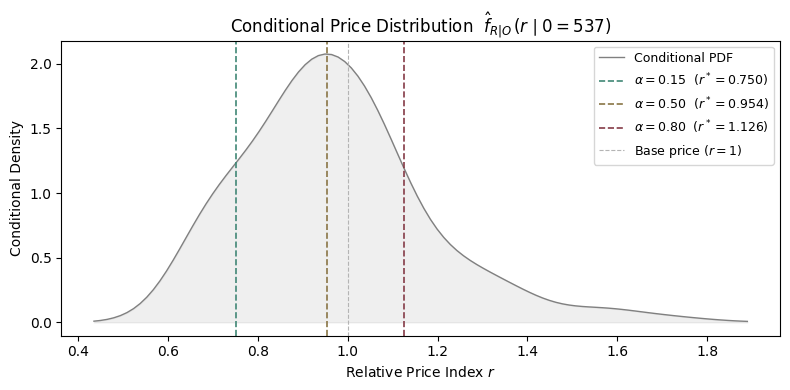
\includegraphics[width=0.8\textwidth]{figures/pricing_quantiles.png}
    \caption{Conditional distribution of relative price indices given forecasted occupancy level $\hat{o}_{12}$.}
    \label{fig:conditional_price_distribution}
\end{figure}

The final recommended price can be obtained as

\begin{equation}
    p_{a,t}^* = r_{t}^* \cdot \bar{p}_{a}
\end{equation}

where $\bar{p}_{a}$ is the apartment-specific base price. As shown in Figure~\ref{fig:conditional_price_distribution}, the choice of $\alpha$ allows for flexibility in the resulting price recommendations, enabling adjustment of pricing strategies according to risk preferences, market conditions, or other relevant factors.

\section{Results and Evaluation}
\label{sec:results}
The model's performance was evaluated on the 30-day hold-out test period. Tables~\ref{tab:generated_price_recommendations} and~\ref{tab:generated_occupancy_recommendations} aim to illustrate the model output for selected apartment ($a=5$) over eight selected days (May 2–9, 2025), using the median quantile $\alpha=0.5$. These examples are mainly intended to show structure of typical output. The full evaluation of the model's performance across all apartments and days in the test period is presented in the subsequent analysis.

\begin{table}[ht]
    \centering
    \small
    \begin{tabular}{|c|c|c|c|c|}
        \hline
        Date       & Relative Price ($\alpha=0.5$) & Recom. Price & Obs. Price & Price Diff. \\
        \hline
        2025-05-02 & 0.9636                        & 1814.37      & 2116.61    & -14.3\%     \\
        2025-05-03 & 0.9823                        & 1849.61      & 2116.61    & -12.6\%     \\
        2025-05-04 & 0.8828                        & 1662.19      & 2116.61    & -21.5\%     \\
        2025-05-05 & 0.7755                        & 1460.27      & 2116.61    & -31.0\%     \\
        2025-05-06 & 0.7795                        & 1467.72      & 2116.61    & -30.7\%     \\
        2025-05-07 & 0.7906                        & 1488.71      & 2116.61    & -29.7\%     \\
        2025-05-08 & 0.9121                        & 1717.40      & 2116.61    & -18.9\%     \\
        2025-05-09 & 0.9557                        & 1799.45      & 2116.61    & -15.0\%     \\
        \hline
    \end{tabular}
    \caption{Relative price recommendations, observed prices, and relative price differences for selected test dates.}
    \label{tab:generated_price_recommendations}
\end{table}

\begin{table}[ht]
    \centering
    \small
    \begin{tabular}{|c|c|c|c|}
        \hline
        Date       & Pred. Occ. & Obs. Occ. & Occ. Diff.(pp) \\
        \hline
        2025-05-02 & 49.8\%     & 61.4\%    & +11.7          \\
        2025-05-03 & 51.6\%     & 59.6\%    & +8.1           \\
        2025-05-04 & 40.7\%     & 29.8\%    & -10.9          \\
        2025-05-05 & 32.3\%     & 40.4\%    & +8.0           \\
        2025-05-06 & 32.7\%     & 43.9\%    & +11.2          \\
        2025-05-07 & 33.7\%     & 45.6\%    & +11.9          \\
        2025-05-08 & 43.3\%     & 45.6\%    & +2.3           \\
        2025-05-09 & 48.8\%     & 50.9\%    & +2.1           \\
        \hline
    \end{tabular}
    \caption{Predicted and observed occupancy with occupancy differences for selected test dates.}
    \label{tab:generated_occupancy_recommendations}
\end{table}

\medskip
For demand forecasting using SARIMA model the Mean Absolute Error (MAE) is 0.0729 and the Root Mean Squared Error (RMSE) is 0.0956. As a reference point, a seasonal naive baseline — which forecasts each day's occupancy as the value observed exactly one week prior — achieves a MAE of 0.0936. The SARIMA model reduces this error by 0.0206, corresponding to a 22.1\% improvement over the naive baseline, confirming that the model provides a meaningful improvement over baseline forecasting method.

A closer examination of the forecast errors reveals a systematic smoothing effect. The standard deviation of predicted occupancy ($0.0835$) is only 64.2\% of the observed standard deviation ($0.1300$), and the Pearson correlation between actual occupancy and signed forecast error is $-0.778$. This indicates that the model compresses the range of demand variation: it systematically over-predicts on low-demand days (mean signed error $+0.0965$) and under-predicts on high-demand days (mean signed error $-0.0248$). The smoothing is inherent to linear time series models and directly propagates into the pricing stage, as the KDE receives a less extreme occupancy input on both peak and trough days.

To assess pricing performance, the model's recommendations at $\alpha=0.5$ are compared to observed transaction prices across all 13 apartments, yielding 290 apartment-day pairs. The recommended price bias is $-4.2\%$, indicating a small systematic tendency to underestimate prices. The mean absolute price error is $28.4\%$, with a standard deviation of $34.7\%$. These results suggest that, while the model captures general pricing tendencies without strong systematic bias, its predictive precision in this basic setup is limited, with a wide range of errors observed across different days and apartments.


\section{Model limitations}
\label{sec:limitations}
The proposed pricing model relies on historical reservation data to estimate the joint distribution of occupancy and relative prices. As a result, the estimated density is limited to the support of the observed data and may not adequately capture rare or extreme demand conditions, which can reduce the reliability of price recommendations in such cases.

Incorporating additional constraints, such as minimum allowable prices or controlled extensions of the distribution support, could improve robustness. This is particularly relevant if the model is combined with alternative demand forecasting approaches that may produce more volatile predictions.

A key component of the model is the SARIMA-based demand forecasting, which provides estimates of future occupancy levels. While the model captures general trends and seasonality, it inherently smooths short-term fluctuations in demand. This can lead to systematic underestimation of peak demand and overestimation during low-demand periods, as observed in the empirical results. Since pricing decisions are directly based on predicted occupancy, these forecasting inaccuracies propagate into the pricing stage and affect the resulting recommendations.

Furthermore, the current model does not incorporate external variables that may influence demand, such as public holidays, weather conditions, local events, or booking lead times. These factors can have a significant impact on short-term accommodation markets and may explain part of the discrepancy between recommended and observed prices. Extending the demand forecasting component to include such variables could improve predictive accuracy and overall pricing performance.

The pricing strategy is controlled by a fixed quantile parameter $\alpha$, which determines the aggressiveness of price recommendations. While this provides a simple mechanism for adjusting pricing behavior, using a constant value over time may not fully reflect changing market conditions or strategic objectives. For example, more conservative pricing may be appropriate for longer booking horizons, while more aggressive pricing may be desirable for medium-term horizons, and again more conservative pricing for last-minute bookings. Allowing $\alpha$ to vary dynamically as a function of time or demand uncertainty represents a potential extension of the model.

Finally, the model operates on data from a specific market segment. Expanding the dataset to include a broader range of apartments, potentially beyond a single provider's portfolio, could improve the estimation of the occupancy–price relationship and enhance the overall performance of the model. At the same time, the choice of dataset plays a critical role: combining data from apartments with significantly different characteristics may distort the estimated relationship and reduce the relevance of the resulting price recommendations. Selecting an appropriate and sufficiently homogeneous market segment, while ensuring reasonable data volume and quality, remains a key challenge in the application of this approach.